\chapter{Medical Imaging and Image Segmentation}
%

The first steps in image-based modeling and simulation involve image acquisition, image processing, and image segmentation. Several techniques are available to produce three-dimensional image data of an anatomical region of interest and are reviewed herein. State-of-the art image processing and image segmentation approaches are summarized in this section as well.

%%%%%%%%%%%%%%%%%%%%%%%%%%%%%%%%%%%%%%%%%%%%%%%
%%%%%%%%%%%%%%%%%%%%%%%%%%%%%%%%%%%%%%%%%%%%%%%
\section{Imaging Approaches}
\label{Imaging Approaches}

Medical imaging is the process of generating discrete image representations of biological tissues. Of the many imaging modalities found in clinical and research settings, the most prevalent are magnetic resonance imaging (MRI) and x-ray computed tomography (CT). Both approaches are \textit{tomographic} in that they produce a series of two-dimensional images representing thin slices through the region, that are subsequently combined to produce a three-dimensional volume representation \cite{larobina_murino_2014}. The data measured during acquisition are different for each modality, and thus the use case typically governs which technique is most appropriate. Several other imaging techniques exist - some of which provide more information than do MRI and CT - and are briefly presented in this section as well. Finally, typical data storage and file formats are discussed.

\subsection{Magnetic Resonance Imaging}
\label{Magnetic Resonance Imaging}

\begin{equation}
\bm{B} = \bm{B}_0 + \bm{g} \cdot \bm{x}
\end{equation}

\begin{equation}
\bm{\omega} = \gamma \bm{B}_0
\end{equation}

\begin{equation}
\bm{\omega} = \bm{\omega}_0 + \gamma \bm{g} \cdot \bm{x}
\end{equation}

MRI provides excellent soft tissue contrast, for tissues such as gray and white matter in the brain, articular cartilage, bone marrow, muscle, and ligaments. Unlike CT, it does not use any harmful ionizing radiation.

resolution
contrast
signal to noise ratio
k space
Fourier transform
magnet
shim coil for homogeneity in magnetic wave from magnet
gradient
RF coils (transmit and receive)
T1, T2, PD
uses
limitations  

\subsection{X-Ray Computed Tomography}
\label{X-Ray Computed Tomography}

houndsfield units

\subsection{Additional Imaging Modalities}
\label{Other Imaging Modalities}

\subsection{File Formats}
\label{Data Format-IMG}

Medical images are typically stored as a combination of a short \textit{header} followed by \textit{pixel data}. The header is typically stored in ASCII format and the pixel data is typically binary. They may be found in the same file or in separate ones. Pixel data is often stored either as a set of two-dimensional images representing each slice, or as a single block of information corresponding to the 3D volume. In either case, data is stored as a 1D array, from which the data can be unrolled based on the axis ordering specified in the header. The header provides metadata to allow software to read and store the image based on the pixel data. Namely, the header contains the matrix dimensions, image resolution, image origin, axis order, data type of the pixel data (i.e., unsigned char, int, etc.), endianness of the pixel data, and data compression encoding (e.g., raw, gzip, bzip2). Additional information may be provided as well, including patient data, image acquisition parameters (e.g., MRI pulse sequence), and date of acquisition. On the clinical side, DICOM (Digital Imaging and Communications in Medicine) files are by far the most popular format for storing medical images, due to it's extensive metadata including patient information and image acquisition protocol. On the research side, several formats are available, including MATLAB~\cite{MATLAB}, NRRD (Nearly Raw Raster Data)~\cite{nrrd}, NIfTI (Neuroimaging Informatics Technology Initiative)~\cite{nifti}, and Analyze~\cite{analyzedirect}. These file formats are different flavors of the general format described above. They are geared more towards image post-processing compared to DICOM, by way of less detailed metadata sections.



%%%%%%%%%%%%%%%%%%%%%%%%%%%%%%%%%%%%%%%%%%%%%%%
%%%%%%%%%%%%%%%%%%%%%%%%%%%%%%%%%%%%%%%%%%%%%%%
\section{Image Segmentation Approaches}
\label{Image Segmentation Approaches}

Arguably the most challenging task in the workflow is the subsequent image processing and \textit{segmenting} of the image of interest.

\begin{figure}[ht]
\centering
\subfigure[]{%
		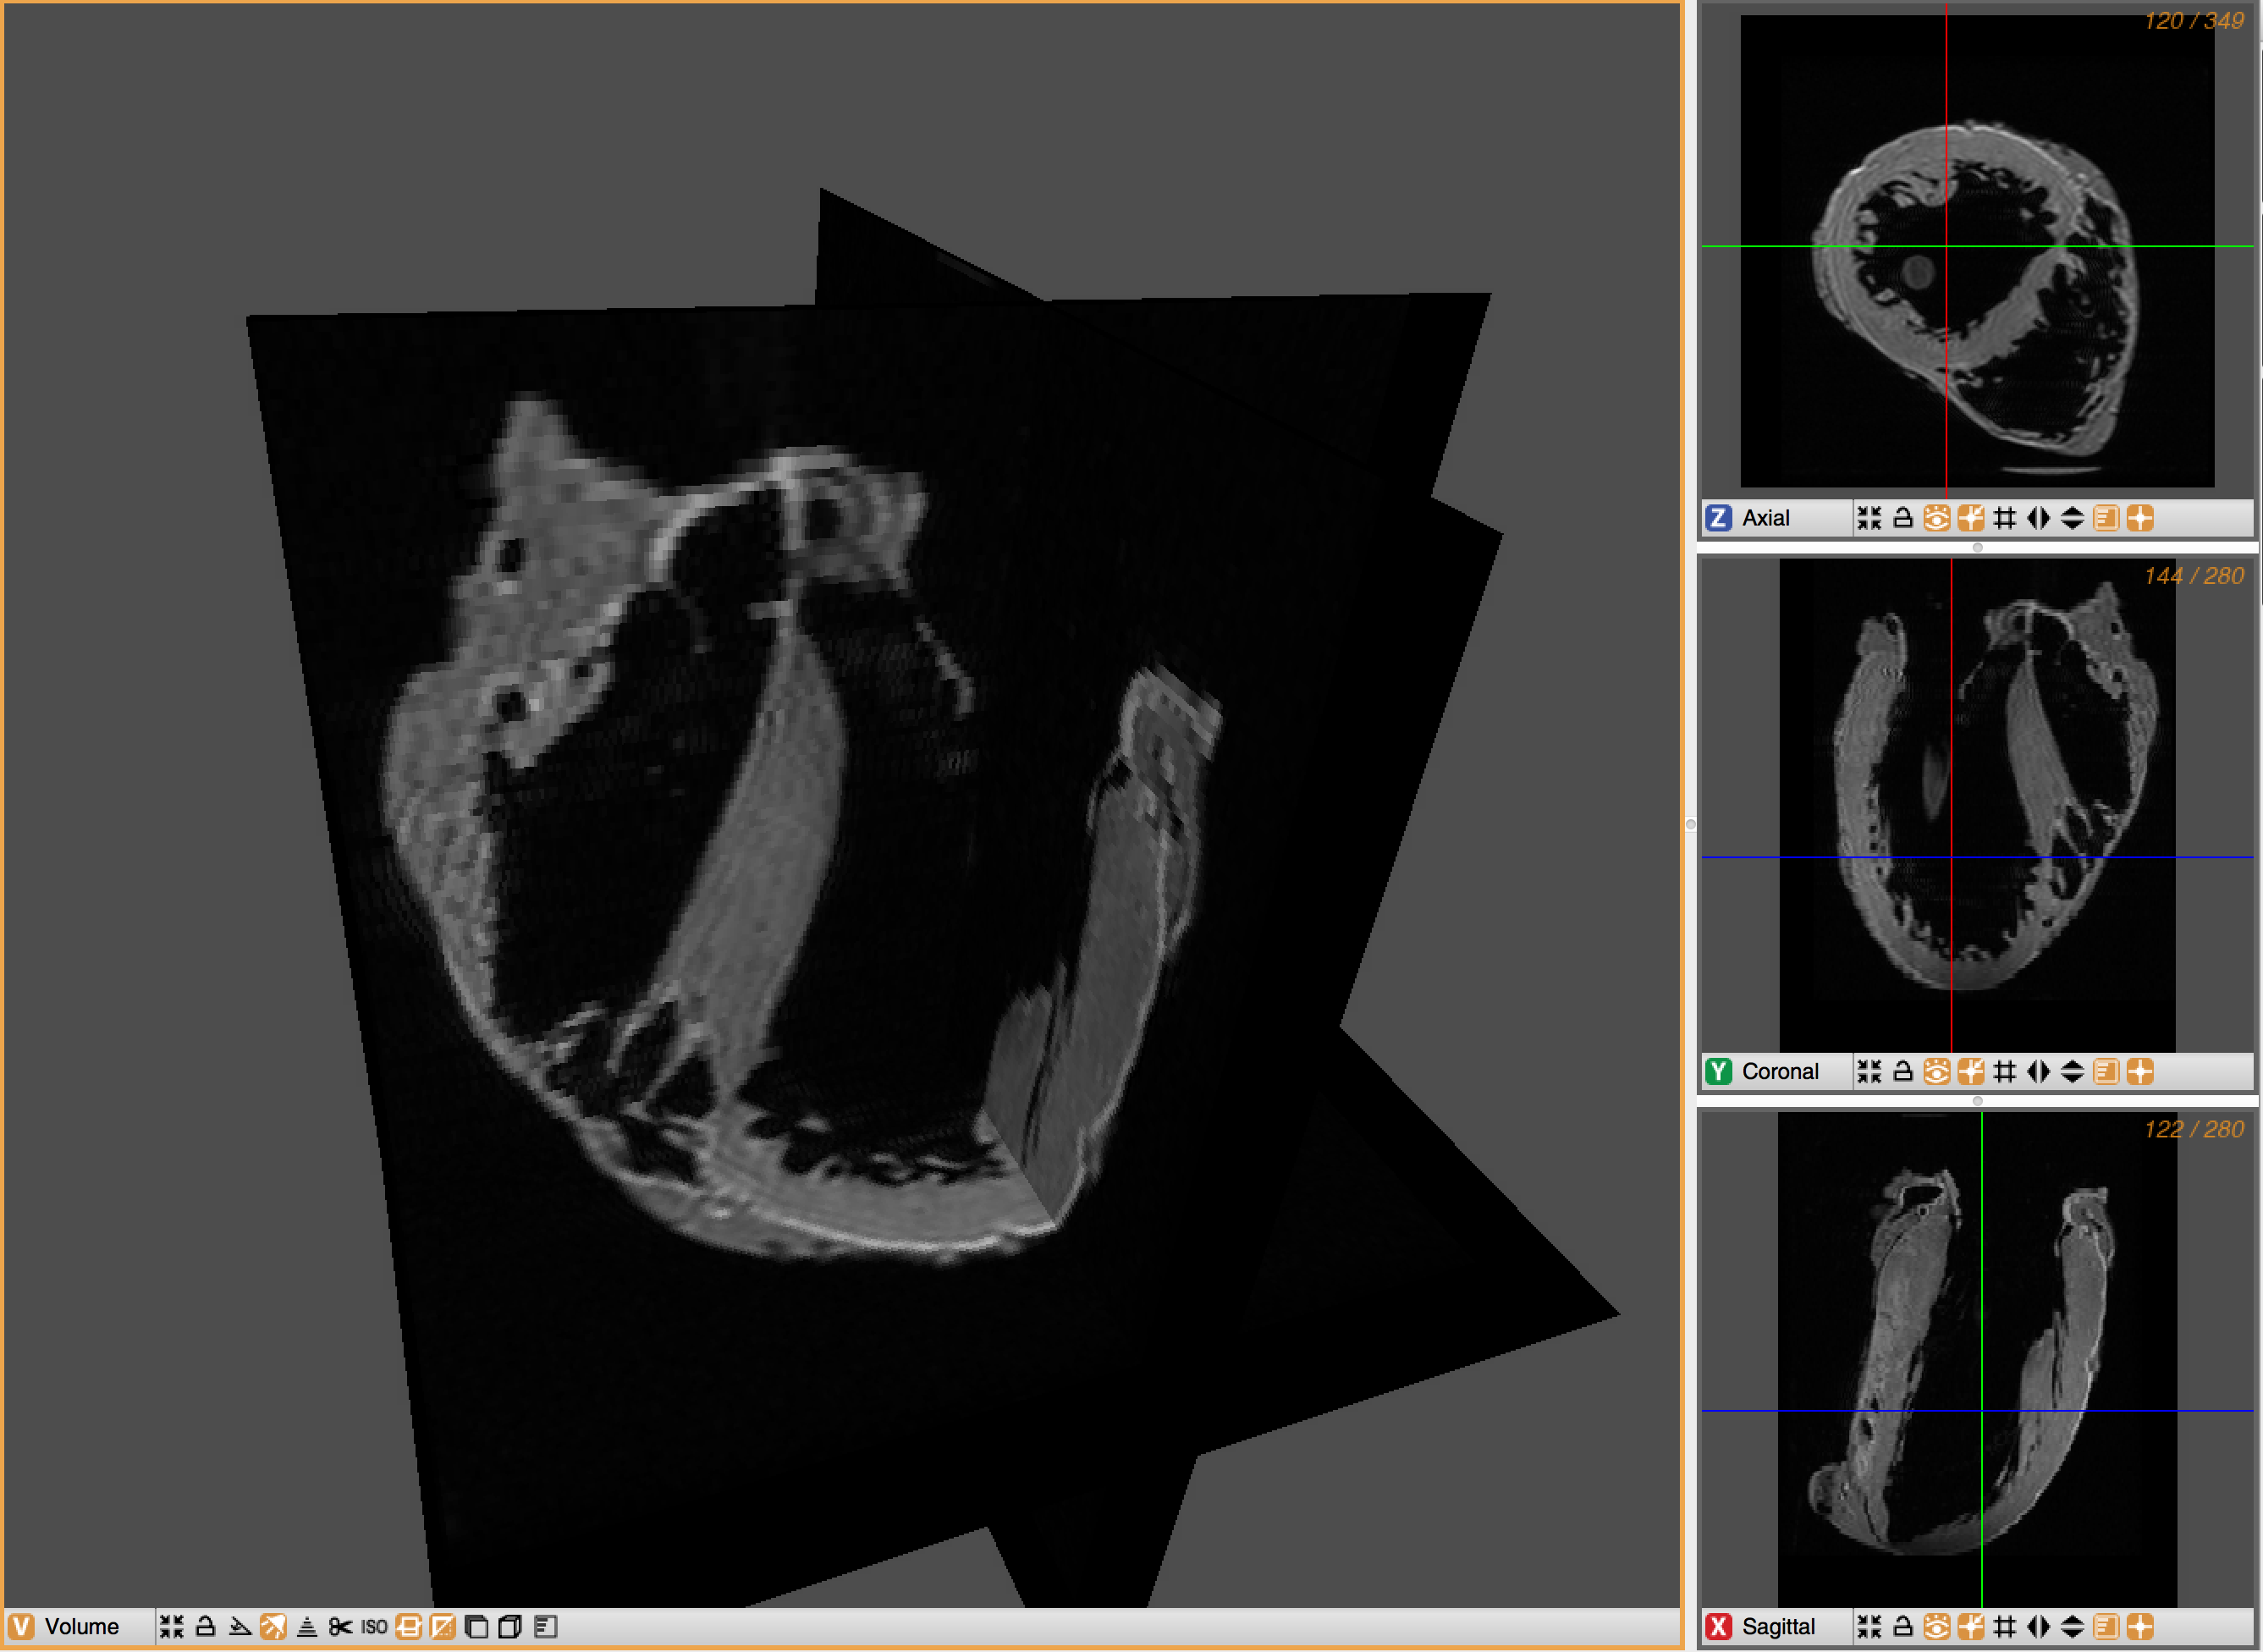
\includegraphics[scale=0.165]{media/1-seg3d/1-raw.png}
\label{fig:seg1}}
\subfigure[]{%
		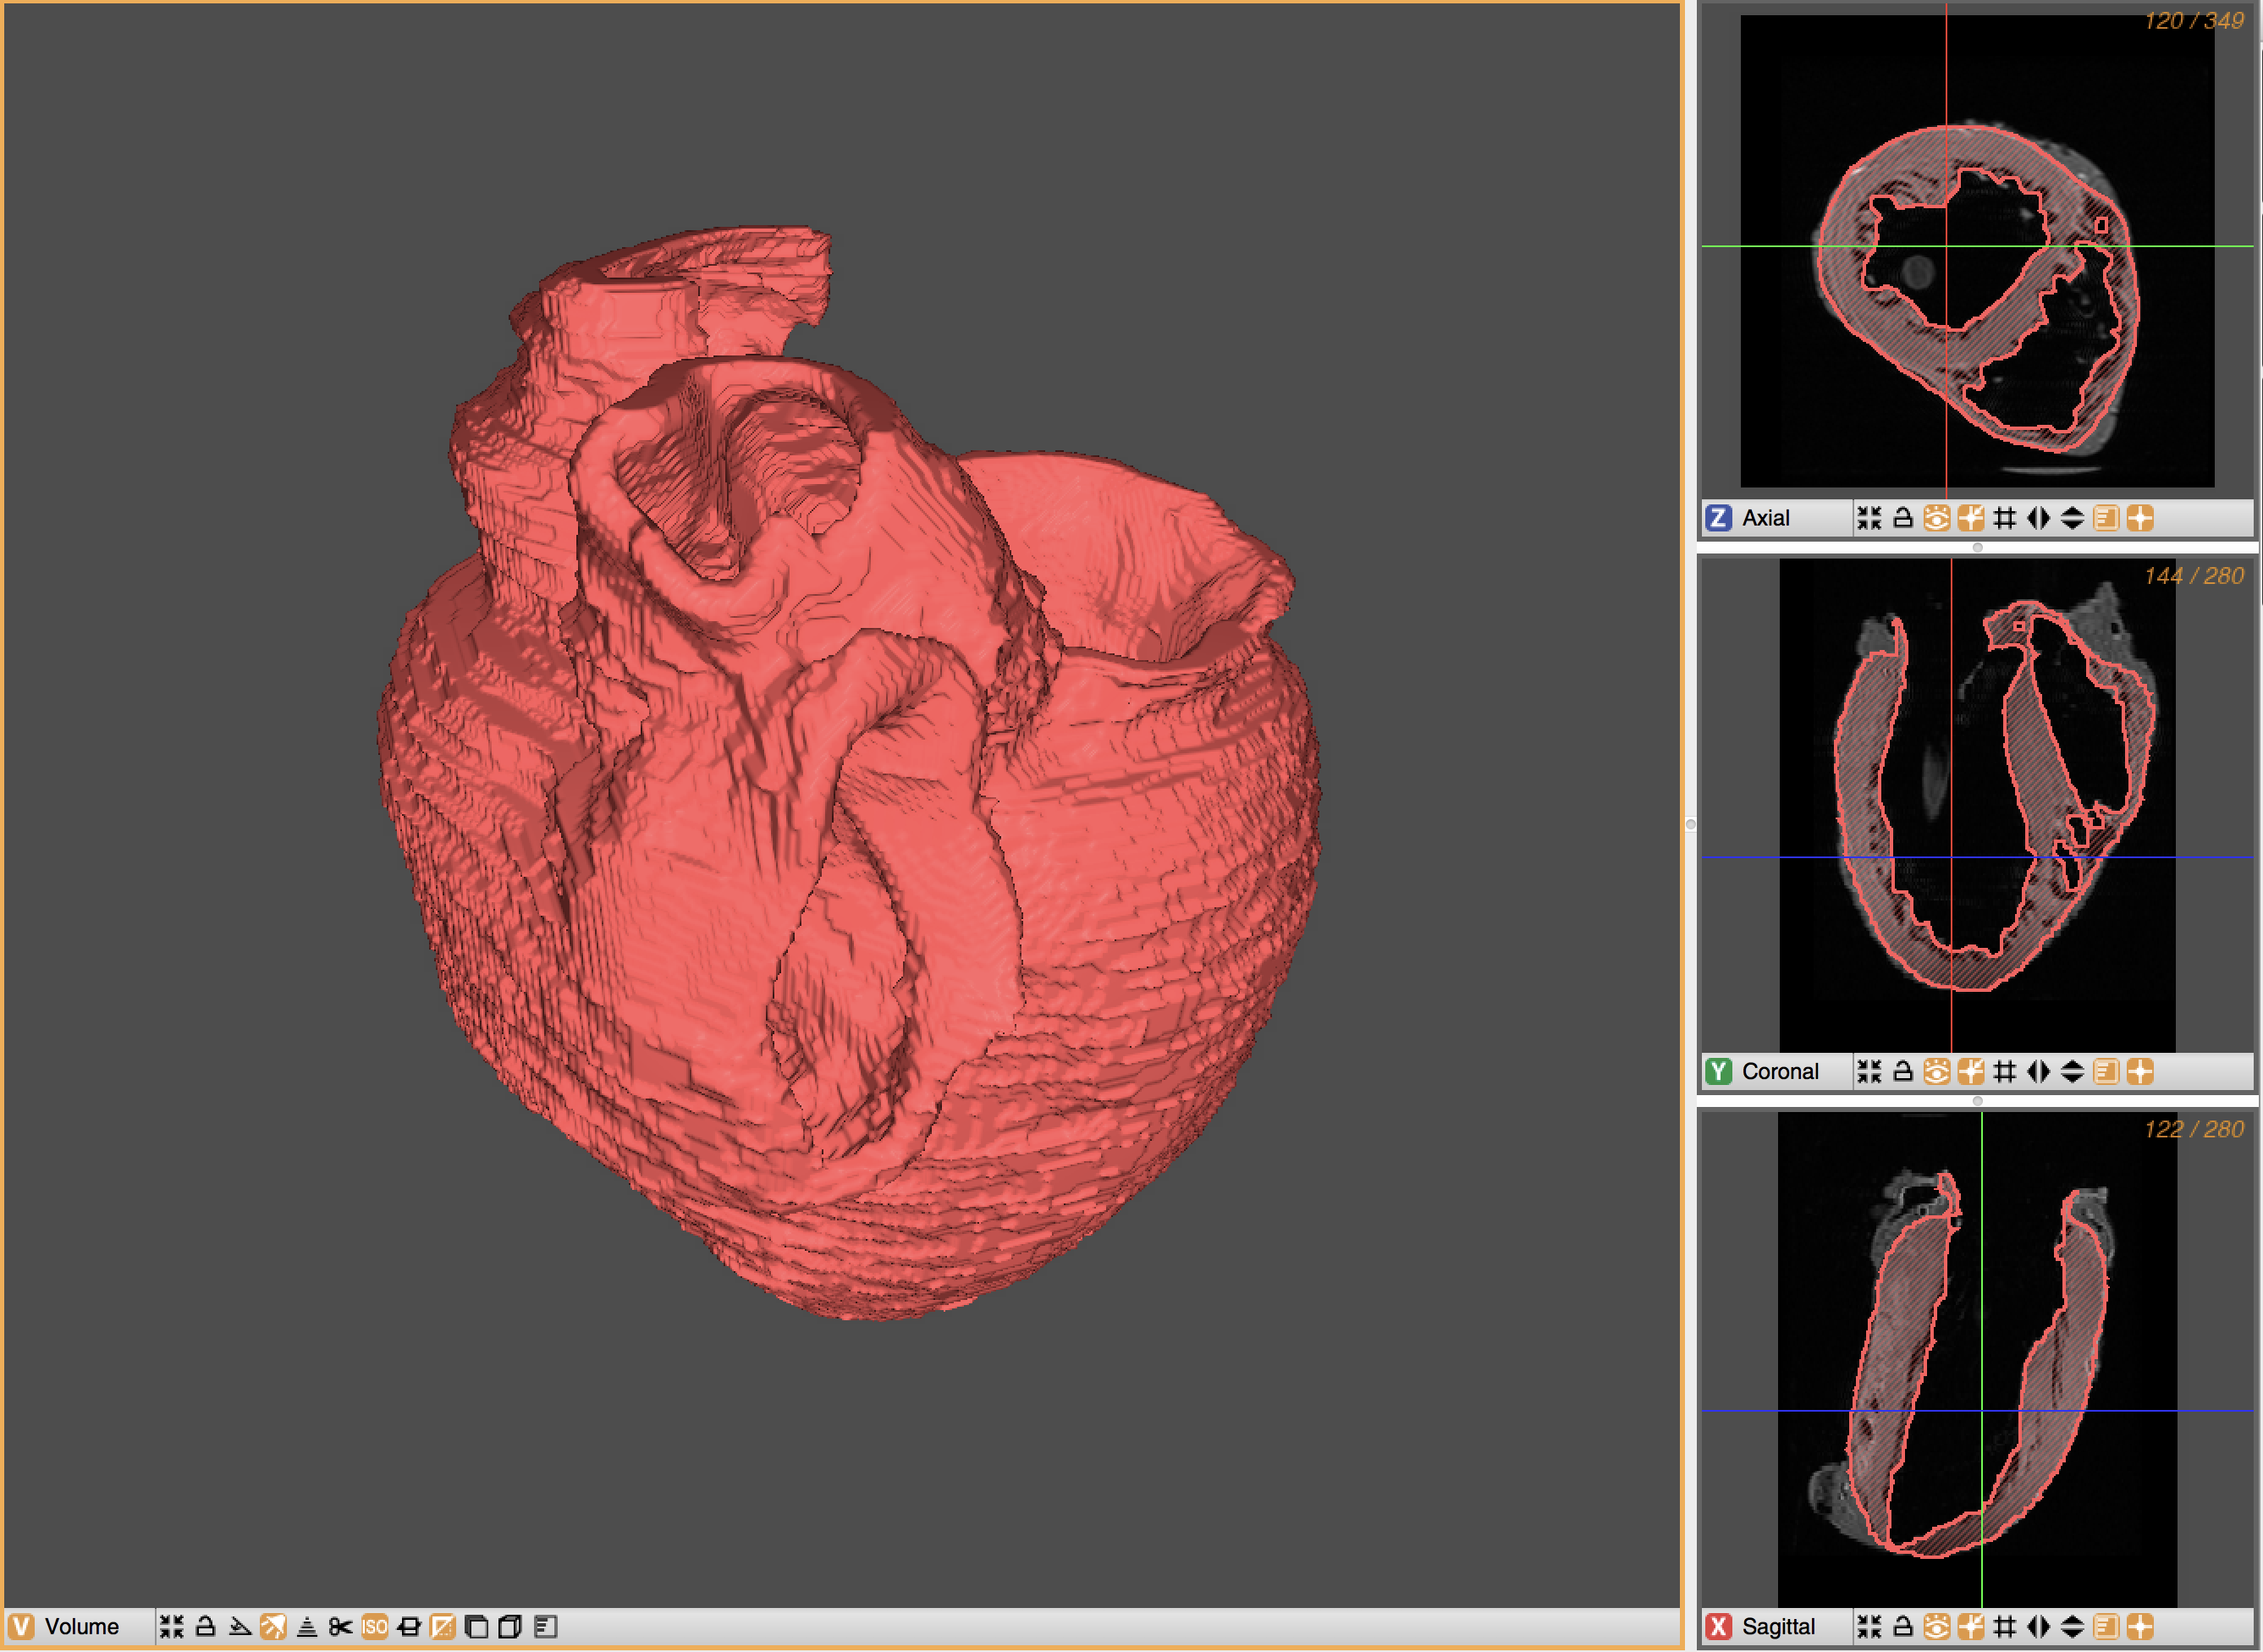
\includegraphics[scale=0.165]{media/1-seg3d/2-seg.png}
\label{fig:seg2}}
%
\caption{(a) MRI of \textit{ex-vivo} human heart, and (b) resulting segmented image mask}
\label{fig:seg}
\end{figure}

Talk about image processing/filtering here. Gaussian blur, mean filter, median filter.

\subsection{Thresholding Methods}
\label{Thresholding Methods}

\subsection{Region-Growing Methods}
\label{Region-Growing Methods}

\subsection{Neural Networks}
\label{Neural Networks}

\subsection{Manual Methods}
\label{Manual Methods}

\subsection{File Formats}
\label{Data Format-SEG}
